% LaTeX .tex example for the proceedings of
% CLIV 3 - III Latin American Wind Engineering Congress
% November, 5-8, 2018, São Paulo, SP, Brazil
%
% Based on the template of the proceedings of COBEM2017 
% MODELO CLIV 3

\documentclass[10pt,fleqn,a4paper,twoside]{article}
\usepackage{cliv}
\usepackage[utf8]{inputenc}
\usepackage[english,portuguese,spanish]{babel}
\usepackage{url}
\def\shortauthor{P. Jabardo, L. Alves, G. Borelli and G. Nader}
\def\shorttitle{Low Cost Anemometers}

\begin{document}
	\fphead
\hspace*{-2.5mm}\begin{tabular}{||p{\textwidth}}
\begin{center}
\vspace{-4mm}
\title{ %CLIV3-2018-XXXX\\
LOW COST ANEMOMETERS FOR WIND TUNNEL AND VENTILATION APPLICATIONS} % (XXXX is the manuscript number)
\end{center}
                  
\authors{Paulo José Saiz Jabardo} \\
\authors{Leandro Alves} \\
\authors{Gabriel Borelli}\\                  
\authors{Gilder Nader}\\
\institution{Instituto de Pesquisas Tecnológicas - Av. Prof. Almeida Prado 532, São Paulo, SP}\\
\institution{pjabardo@ipt.br, leoalvs@ipt.br, gborelli@ipt.br, gnader@ipt.br} \\
\\
\abstract{\textbf{Abstract.} Low cost and simple constant current and pulsed constant temperature anemometers are described. The proposed anemometers use a self-heated thermistor as a flow sensor and very simple electronics are used. Data acquisition and control use commonly available micro-controllers. A simple heat transfer model is used to simulate the main characteristics of the sensor and laboratory tests show that the calibration curves of the sensors are repeatable and even though the sensor has a spherical shape, a directional sensitivity is noticeable. }\\
\\
\keywords{\textbf{Keywords:} anemometer, wind tunnel, ventilation, constant current, constant temperature}\\
\end{tabular}

\section{INTRODUCTION}

Thermal anemometers are very common in wind engineering and ventilation. In particular its ability to measure very low wind speeds is a distinctive advantage when compared to Pitot tubes. Depending on sensor element dimensions, very high frequencies and speeds can be measured as well. Two simple thermal anemometers using small thermistors as sensors are proposed and analyzed. The objective of this work is to develop low cost and simple arrays of velocity probes using readily available micro-controllers for data acquisition. A further objective is to find a replacement of the Irwin probes for pedestrian level wind measurements.

While thermal anemometers are common, they usually consist of  hand held versions and are not very suitable for making sensor arrays. Some models cost US\$50 a unit, but quality meters usually cost US\$200 or more. Arrays of rugged \emph{and} disposable sensors that can be easily installed inside wind tunnel models are harder to come by.


\section{MODELING THERMAL ANEMOMETERS}

The loss of heat of a warm body exposed to air depends on the velocity of the air: the higher the velocity, the larger the heat loss. Newton's law of cooling provides a simple, empirical relationship for the heat loss \citep{Incropera96}. On the other hand, if an electric current is passing through the body, heat is generated according Joule's law of heating. These two phenomena, along with thermal inertia of the body results in a differential equation for the temperature of the body:

\begin{equation}
  mc_p\frac{dT}{dt} = -h\cdot A\cdot \left(T - T_a\right) + R\cdot i^2
  \label{eq:temp}
\end{equation}

In this equation $T$ is the temperature of the body, $m$ is its mass and $c_P$ its specific heat. The convection coefficient is given by $h$, $A$ is the external surface area of the heated body and $T_a$ is the room temperature. Finally, $R$ is the electric resistance of the body and $i$ is the electric current circulating through it.

This simplified model assumes that the temperature of the body is uniform. This is valid if the Biot number $Bi = hL/k$ is small enough (where $k$ is the thermal conductivity of the body and $L$ is a typical dimension). As it will be seen later, this hypothesis is not always true. A major drawback in this model is the value of the convection coefficient $h$: it is not known but it strongly depends on the fluid velocity. While the literature abounds with correlations for the convection coefficient, most of them have high uncertainty and are valid for very specific geometries. The practical result of these observations is that thermal anemometry can not be  a primary standard for fluid velocity: a calibration will always be necessary. But this simple model and literature correlations are enough to understand the behavior and design a thermal anemometer.

Equation \ref{eq:temp} can be used in several ways to implement a thermal-anemometer but usually, the anemometer depends on the variation of electrical resistance ($R$) with temperature. Most solids present, in a wide range of temperature around room temperature, a linear relationship between resistance and temperature where the resistance gradually increases with temperature. Some semiconducting materials, on the other hand, might present strong, nonlinear, variations of resistance with temperature which, while presenting a more complicated behavior, also responds much better to small variations in temperature. These materials are often called \emph{thermistors} and often have a negative temperature coefficient (NTC), i.e., the resistance decreases with increasing temperature. The anemometers developed in this study use NTC thermistors as sensor elements. A semi-empirical relationship between resistance and temperature is given by the following equation \citep{Sandborn72}:
\begin{equation}
  R = R_0 \cdot e^{B\cdot\left(\frac{1}{T} - \frac{1}{T_0} \right)}
  \label{eq:thermistor}
\end{equation}
where $R_0$ is the resistance of the thermistor at the reference temperature, usually $293.15\:K = 20^\circ C$ and $B$ is an empirical coefficient which varies for different thermistors.

\begin{figure}[h!]
\centering
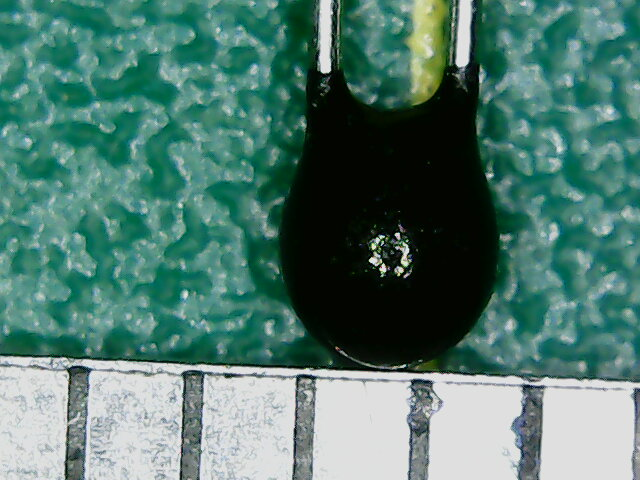
\includegraphics[width=0.45\textwidth]{../../figures/termistor.jpg}
\caption{Photo of a thermistor with an approximate diameter of 2 mm. $R_0 = 5\:k\Omega$ and $B = 3000\:K$}
\label{fig:thermistor}
\end{figure}

Thermistors come in all sizes and shapes. Figure \ref{fig:thermistor} shows a photograph of a thermistor with an approximate diameter of 2 mm. Its spherical overall shape suggests that it can be used as an omni-directional probe. It will be shown later that this specific thermistor has a directional sensitivity which can not, be simply discarded.

The strong dependence of resistance on temperature and its small dimensions make the thermistor shown on figure \ref{fig:thermistor} a strong candidate for an anemometer sensor element. In steady flow, equation \ref{eq:temp} reduces to:
\begin{equation}
  R(T)\cdot i^2 = h(U)\cdot A \cdot \left(T - T_a\right)
  \label{eq:anemo}
\end{equation}
There are two common ways to use this equation to measure velocity:
\begin{itemize}
\item Constant Current (CCA)
\item Constant Temperature (CTA)
\end{itemize}
Today, most hot wire anemometers are CTA but CCA has wide use still. We will analyze both since simple circuits using both principles are suggested.

\subsection{Constant Temperature Anemometer (CTA)}
For now, no mechanism is proposed on how to keep the temperature constant. But if the temperature is constant, so is the resistance. An operating temperature is selected ($T_w$) and the circuit tries to keep the resistance constant equal to $R_w = R(T_w)$. The voltage ($E_0$)  across the sensor element is, according to eq. \ref{eq:anemo}:
\begin{equation}
  E_0 = \sqrt{R_w h A \left(T_w - T_a\right) }
  \label{eq:cta}
\end{equation}

\begin{figure}[h!]
  \centering
  \begin{tabular}{cc}
    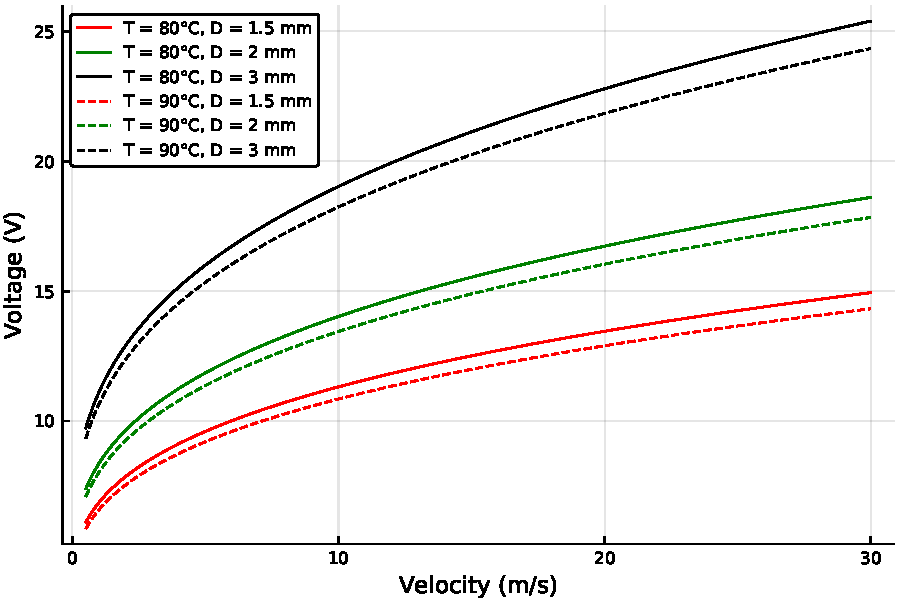
\includegraphics[width=0.45\textwidth]{../../figures/CTA-Eo.pdf} & 
    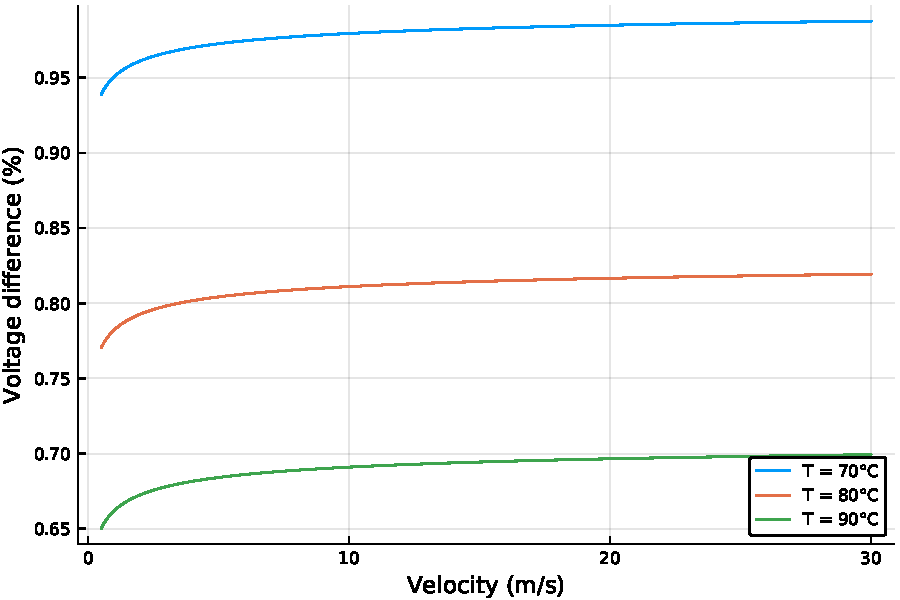
\includegraphics[width=0.45\textwidth]{../../figures/CTA-dt.pdf} \\
    \parbox{0.4\textwidth}{\footnotesize (a) Effects of diameter and operating temperature on anemometer output} & \parbox{0.4\textwidth}{\footnotesize (b) Effects of $1^\circ C$ increase of room temperature ($T_a$) on anemometer output}\\
  \end{tabular}
  \vspace{0.4cm}
\caption{Simulation of a  a constant temperature anemometer for different diameters and operating temperatures ($T_w$). $R_0 = 5\:k\Omega$ and $B = 3000\:K$}
\label{fig:cta1}
\end{figure}

Figure \ref{fig:cta1}a shows the response of a constant temperature anemometer for different operating conditions. It is clear that the diameter has a large effect on the output. The power (and voltage) required is much larger but the sensitivity isn't any better. The operating temperature also affects the power requirements but higher operating temperatures present an advantage: the effect of room temperature variation is smaller as shown on figure \ref{fig:cta1}b where the effect of a $1^\circ C$ room temperature increase is shown as anemometer output difference.

\subsection{Constant Current Anemometer (CCA)}

When operating at constant current, the temperature will vary, even though the current is constant. In this case, no simple explicit expression for the output voltage exists and a nonlinear algebraic equation must be solved for each wind velocity. Figure \ref{fig:cca1} shows the general behavior of the constant current anemometer.

\begin{figure}[h!]
\centering
% 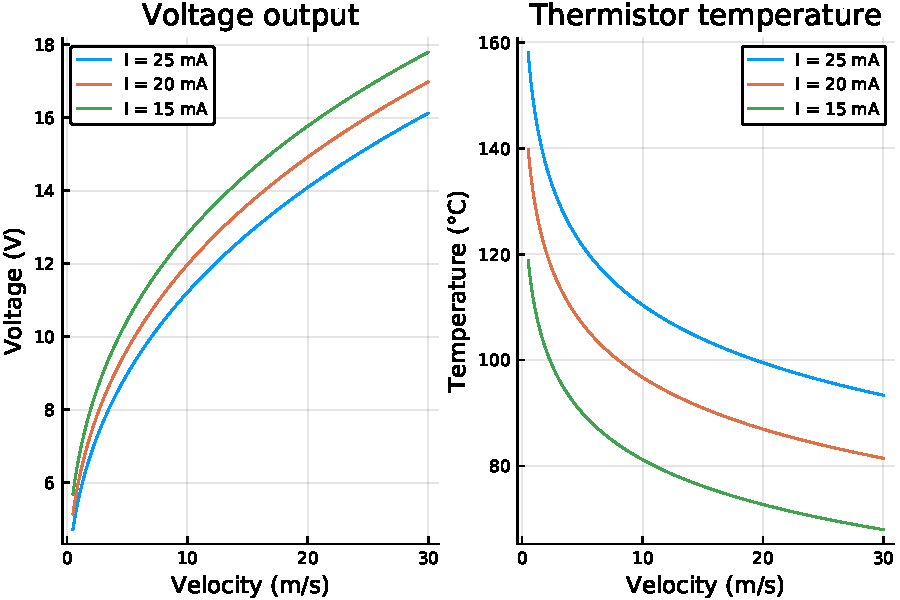
\includegraphics[width=0.8\textwidth]{../../figures/CCA.pdf}
  \begin{tabular}{cc}
    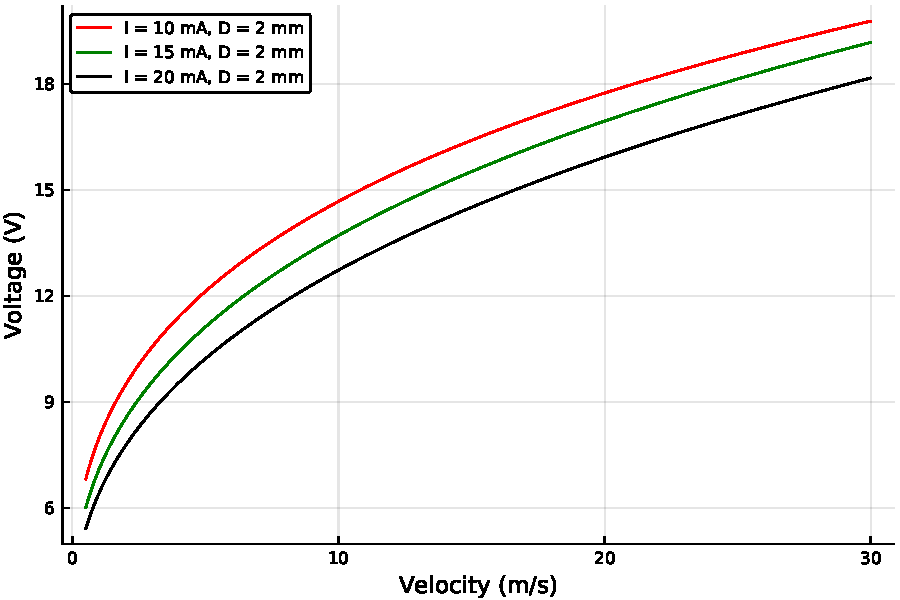
\includegraphics[width=0.45\textwidth]{../../figures/CCA-Eo.pdf} & 
    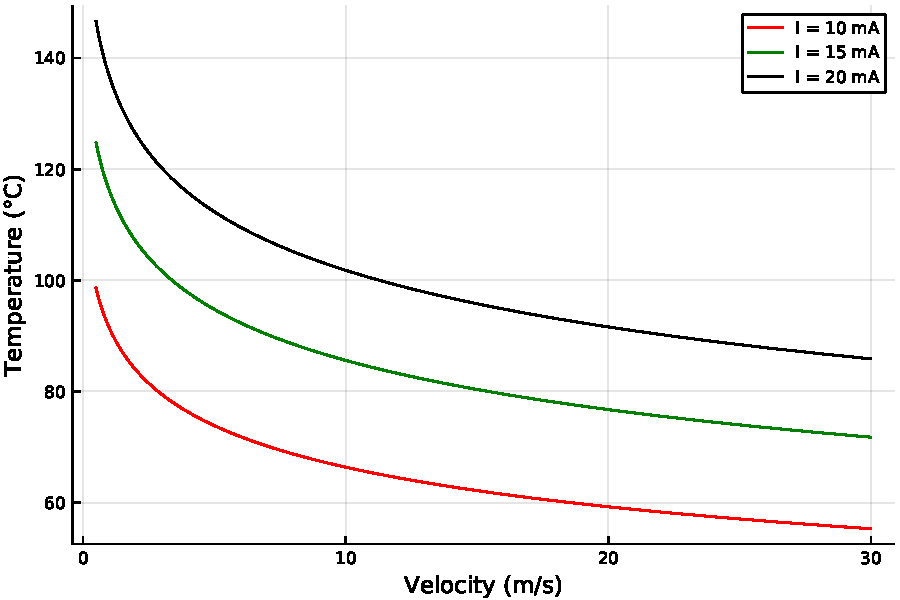
\includegraphics[width=0.45\textwidth]{../../figures/CCA-T.pdf} \\
    \parbox{0.4\textwidth}{\footnotesize (a) Effects of probe current on anemometer output} & \parbox{0.4\textwidth}{\footnotesize (b) Temperature of a thermistor for constant current operation}\\
  \end{tabular}
  \vspace{0.4cm}

\caption{Simulation of a constant current anemometer for different currents. $R_0 = 5\:k\Omega$ and $B = 3000\:K$}
\label{fig:cca1}
\end{figure}

The output voltage of the CCA behaves as expected (figure \ref{fig:cca1}a) but there one important aspect: the temperature increases significantly for lower velocities (figure \ref{fig:cca1}b). Since the thermistor used has a maximum operating temperature of 120 $^\circ C$, a burn out of the sensor is a real possibility if the currents are high or the sensor is used in a small confined space. These high temperatures may also change the calibration curve. Since the operating temperature changes considerably with wind speed, corrections due to room temperature ($T_a$) are more complicated and can be large for higher speeds.

\subsection{Time constant of the sensor}

Up to this point, a steady flow and a stable anemometer was assumed. If the flow velocity changes, the response of the anemometer will depend on the dynamics of the sensor. This dynamics is also important when designing the circuit. The simplest way to assess the dynamics of the sensor is to estimate how long it takes for the sensor to cool down from a given higher than room temperature. The time constant depends on the velocity and using equation \ref{eq:temp} with fixed $h$, a time constant of the order of 1 s  is obtained. The time that it takes for the temperature difference to drop 10\% is given by
\begin{equation}
  \tau = -\ln(0.9) \cdot \frac{m\cdot c_p}{h\cdot A}
  \label{eq:timeconst}
\end{equation}
For $U=10\:m/s$, $\tau \approx 0.5\:s$.


\section{THE ELECTRONICS OF THE LOW COST ANEMOMETERS}
The idea behind this project is the design of low cost and easy to manufacture anemometers. If arrays of sensor are to be used, it is interesting to have a simple computer data acquisition system. This project uses the NodeMCU 32s micro-controller board to control and acquire data from the anemometer. This board has 16 analog 12 bit inputs and several other digital inputs/outputs. Besides USB communication, the NodeMCU board has both built-in wi-fi and Bluetooth. The development environment is the same one used by Arduino so that reference materials are easily available.

\subsection{The Constant Current Anemometer}
The low time constant of the thermistor and the low current involved makes it possible to use commonly found integrated circuits (IC) to generate a constant current source. The LM317LZ is a cheap, easy to use and widely available voltage regulator that can be easily used to design a constant voltage current source. This IC tries to maintain a constant voltage of 1.25 V between its output and adjust terminals but with a resistor it can be used as a constant current source. Figure \ref{fig:electronics} shows the circuit that implements the anemometer. The 82 $\Omega$ resistor ensures an output current of approximately 15 mA. Since the output voltage can be as high as 20 V and the analog inputs of the micro-controller are limited to 3.3 V, a voltage divider is used to ensure a lower voltage at the analog input of the NodeMCU 32s.


\begin{figure}[h!]
  \centering
  \begin{tabular}{cc}
    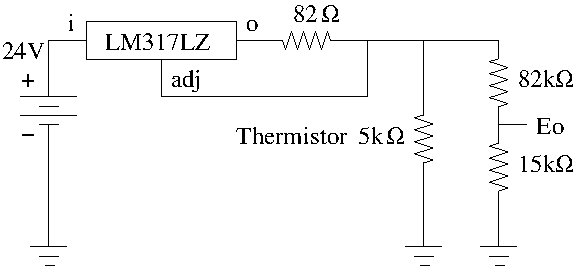
\includegraphics[width=0.46\textwidth]{../../figures/cca.pdf} &
    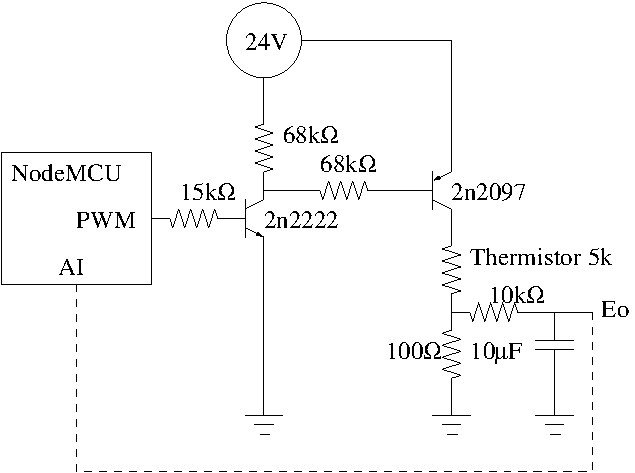
\includegraphics[width=0.46\textwidth]{../../figures/cta.pdf} \\
    (a) Constant current anemometer (CCA) & (b) Pulsed constant Temperature anemometer (PCTA)\\
  \end{tabular}
  \vspace{0.5cm}
  \caption{Anemometer electronic circuits }
\label{fig:electronics}
\end{figure}



\subsection{The Pulsed Constant Temperature Anemometer}

A typical constant temperature anemometer uses analog electronics to implement the feedback control of the temperature. The electronics for this feedback control can be quite complicated for a non-expert. The usual approach is to use a Wheatstone Bridge that is balanced when the sensor resistance equals the preset operating resistance ($R_w$). When the resistance drifts off, the bridge is unbalanced and this unbalance is used to control the input to of bridge. The general layout can be seen in \citet{Lomas86} and a specific implementation is provided by \citet{Palma16}. Even though the large time constant of the thermistor and large resistance change with temperature may allow for a simpler circuit, its design and implementation is much more complicated than the constant current anemometer proposed here for instance. Another approach is to implement the control in the micro-controller using high level language programming. Most micro-controller do not have analog output. But they do have PWM output. Pulse Width Modulation (PWM) is a rectangular wave with constant frequency and amplitude where the percentage of time the pulse is at a high voltage can be varied between 0\% (always off) and 100\% always on.

The idea behind the pulsed constant temperature anemometer (PCTA) is to control the percentage of time current is fed from a constant voltage source (in this case a 24 V easily available source). The control variable is the fraction of time $x$ that the circuit is on (therefore, $0 \le x \le 1$). The PCTA was implemented using the circuit shown in figure \ref{fig:electronics}b. The transistors in this circuit operate in saturation so they work in on/off conditions depending on the instantaneous output of the PWM signal from the controller. The circuit is basically used to turn on and off the current to the thermistor.

If the resistance of the thermistor starts to fall, its temperature is increasing and $x$ should be lowered. On the other hand, if the resistance rises, the temperature is increasing and $x$ should be increased.

The trick is to measure the resistance. This done by a low pass filter that measures the current on a small resistor in series with the thermistor. If the PWM frequency is high, the output from the filter will oscillate slowly and the mean current is given by $i = Eo / 100\Omega$. With this information, the thermistor resistance can be estimated as:

\begin{equation}
  R = 100\Omega\cdot\left( x \frac{24V}{E_o} - 1 \right)
  \label{eq:Rt}
\end{equation}

This can be compared to the expected resistance of the thermistor $R_w = R(T_w)$. Since the response of the thermistor is slow, this can be easily accomplished in commonly available micro-controllers which will adjust the PWM accordingly ($x$).

It is interesting to note that since in steady state the stable value of $x$ varies with the velocity of the fluid, a simple proportional controller will operate very poorly. A digital Proportional/Integral controller was implemented to keep the resistance constant.

\section{RESULTS AND DISCUSSION}

Both anemometers constructed where calibrated and a few tests where carried out. Figure \ref{fig:calibr-cca} shows the results for the CCA. The calibration is repetitive and when large change of velocity occurs (both up and down), the sensor responds accordingly. The sudden downward change in velocity was obtained by shutting off a 25 m/s flow. The upward step change in velocity was obtained by rapidly moving the sensor into a 25 m/s flow. In the case of the CTA (figure \ref{fig:calibr-cta}), the calibration curve is still good but not as good as observed for the CCA. When large change in velocities occur, the controller implemented has some difficulty for a while but recovers after a few seconds. The tuning of the PI controller is an on going work and better results are expected. The calibrations where carried out using the Dantec Dynamics calibrator.

Even though the thermistor has a general spherical shape the probe is not omni-directional as is shown in figure \ref{fig:calibr-dir}. A support used for directional calibration of 3D hot wire probes was used to vary the wind incidence. There is a 30\% variation in velocity depending on the orientation. It is interesting to note both cusps on the curve. These directions happen to coincide with flow parallel to the plane formed by the thermistor lead (flow parallel to photo shown in figure \ref{fig:thermistor}). While asymmetries in the shape and flow around the thermistor can cause some directional sensitivity, the presence of the abrupt cusps in the curve suggests that the internal current flux inside the thermistor is the cause to the directional sensitivity. Further research using numerical simulation is ongoing to better understand this result.

\begin{figure}[h!]
\centering
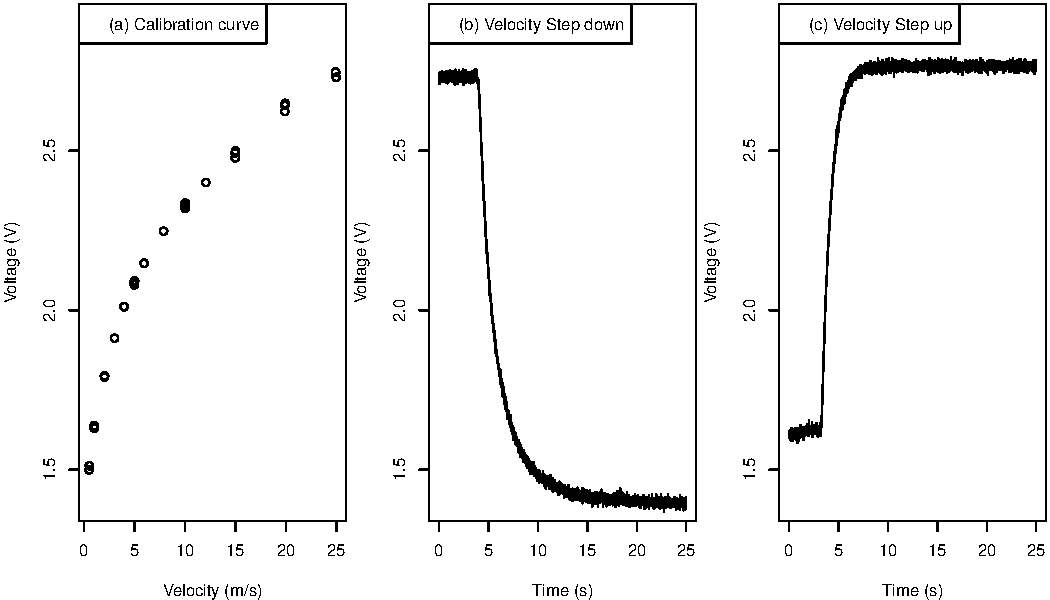
\includegraphics[width=0.75\textwidth]{../../figures/cca-cal.pdf}
\caption{Calibration curves and step down and step up velocity changes for the constant current anemometer}
\label{fig:calibr-cca}
\end{figure}


\begin{figure}[h!]
\centering
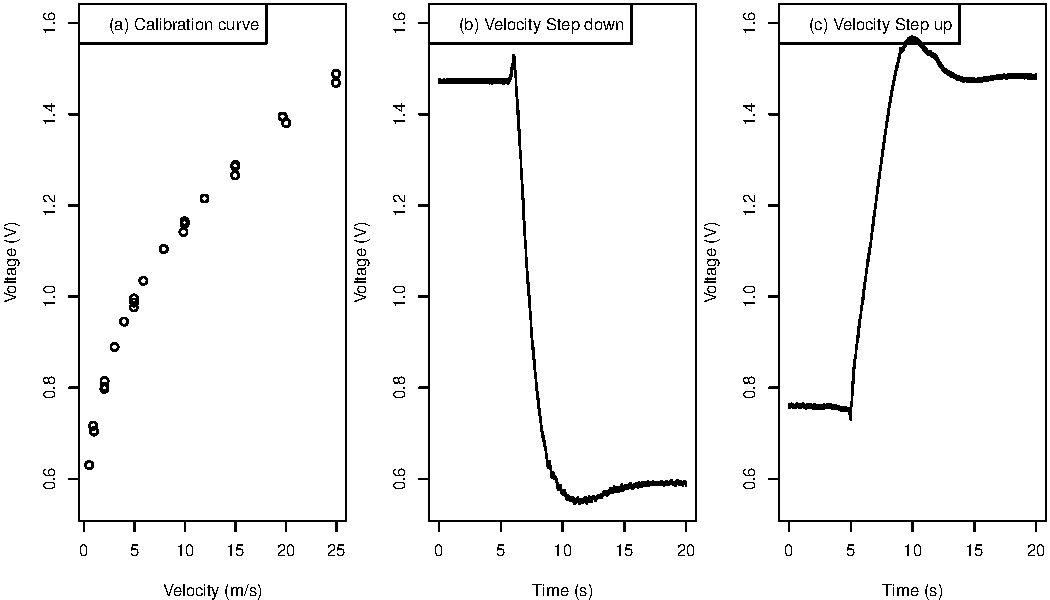
\includegraphics[width=0.75\textwidth]{../../figures/cta-cal.pdf}
\caption{Calibration curves and step down and step up velocity changes for the pulsed constant temperature anemometer}
\label{fig:calibr-cta}
\end{figure}

\begin{figure}[h!]
\centering
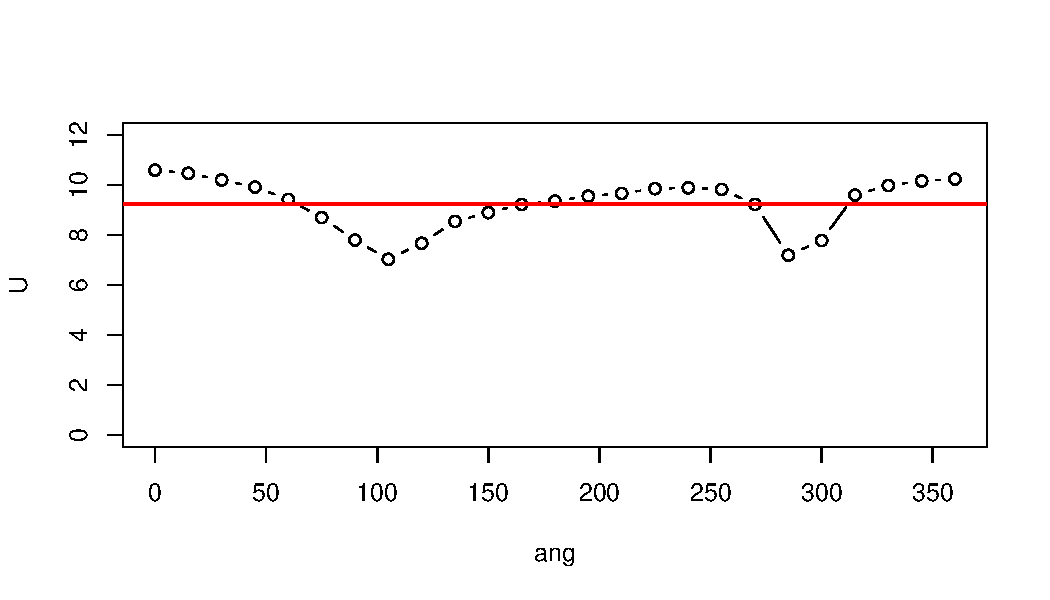
\includegraphics[width=0.65\textwidth]{../../figures/dircal.pdf}
\caption{Directional calibration of the anemometer}
\label{fig:calibr-dir}
\end{figure}

\section{CONCLUSIONS}
Two different, simple and cheap circuits to measure air velocity were proposed and analyzed. The calibration curves showed little dispersion which indicates that both circuits have potential. The ability to build cheap arrays velocity sensors opens up several possibilities in wind engineering and ventilation, both in the wind tunnel and in field measurements. The cost of the micro-controller is around US\$20 in Brazil and each sensor costs and additional US\$2 with the possibility of using 12-16 sensors per micro-controller. Manufacturing requires elementary soldering capabilities. 

The controller of the constant temperature anemometer could certainly see some improvement. An issue that was not dealt up to this point is the effect of changes in room temperature. Since the operating temperature is low (much lower than typical operating temperature of research hot wire systems), the effect of changes in room temperature will be more significant. The expression suggested by \citet{Jorgensen02} can be used for the PCTA but an expression using the calibration curve of the sensor itself could be developed (the calibration curve is a sort of convection coefficient curve). In the case of the constant current sensor, the variation of operating temperature with velocity introduces complications but an approximate temperature correction might be possible.

It is not clear if the sensitivity to direction is due to geometry or the internal structure of thermistor which causes asymmetric heat exchange. Perhaps a simple probe support could improve this. The cusps visible in figure \ref{fig:calibr-dir} suggest that the current flux between the thermistor leads is responsible. If that is the case, thermistors with different shapes, where leads arrive and leave in the same direction could solve part of the directional sensitivity. This problem will require further research. While e 30\% variation is not too large, without further studies, this probe can not simply replace the Irwin probe \citep{Irwin81} for \emph{mean} pedestrian level velocity measurements. 

This project is open sourced and any contributions are welcomed. See \url{https://github.com/pjabardo/ThermistorHW.jl} for further developments.

\section{REFERENCES} 

\bibliographystyle{cliv}
\renewcommand{\refname}{}
%\bibliography{bibfile}
\bibliography{bibanem}

\section{RESPONSIBILITY NOTICE}

The authors are the only responsible for the printed material included in this paper.

\end{document}
